\documentclass{beamer}

% \usetheme{Singapore}
% \usetheme{Malmoe}
\usetheme{Warsaw}

\usepackage[utf8]{inputenc}
\usepackage[russian]{babel}
\usepackage{cmap}
\usepackage{mathrsfs}
\usepackage{changepage}
\usepackage{xcolor}
\usepackage[noend]{algpseudocode}
\usepackage{tikz}

% \useoutertheme{split}
\useoutertheme{shadow}
\usefonttheme{professionalfonts}
\usepackage{graphicx}
\usepackage{psfrag}
\beamertemplatenavigationsymbolsempty 
\DeclareMathOperator{\sign}{sign}

\setbeamertemplate{footline}[frame number]

\author{Павел Филонов \\ \href{mailto:filonovpv@gmail.com}{filonovpv@gmail.com}}
\title{Введение в машинное обучение}
\subtitle{Логические методы классификации}

\begin{document}
\begin{frame}[plain]
    \titlepage
\end{frame}
\begin{frame}[plain]{Содержание}
  \tableofcontents
\end{frame}

\section{Решающие деревья}
\begin{frame}{Определение решающего дереве (Decision Tree)}

{\it Решающее дерево} --- алгоритм классификации $a(x)$, задающийся деревом (связным ациклическим графом):
\begin{enumerate}
    \item $V = V_{\text{внутр}} \sqcup V_{\text{лист}},\; v_o \in V$ --- корень дерева;
    \item $v \in V_{\text{внутр}}$: функции $f_v: X \rightarrow D_v$ и $S_v : D_v \rightarrow V,\; |D_v| < \infty$;
    \item $v \in V_{\text{лист}}$: метка класса $y_v \in Y$.
\end{enumerate}

\begin{columns}
\column{0.5\textwidth}
Алгоритм работы решающего дерева:
\begin{algorithmic}
    \State $v \gets v_0$
    \While {$v \in V_{\text{внутр}}$}
        \State $v \gets S_v(f_v(X))$
    \EndWhile
    \State\Return $y_v$
\end{algorithmic}

\column{0.5\textwidth}
\includegraphics[width=\textwidth]{fig/DT-crop.pdf}
\end{columns}
\end{frame}

\begin{frame}{Пример решающего дерева}
Задача Фишера о классификации цветков ириса на 3 класса

\begin{columns}
\column{0.5\textwidth}
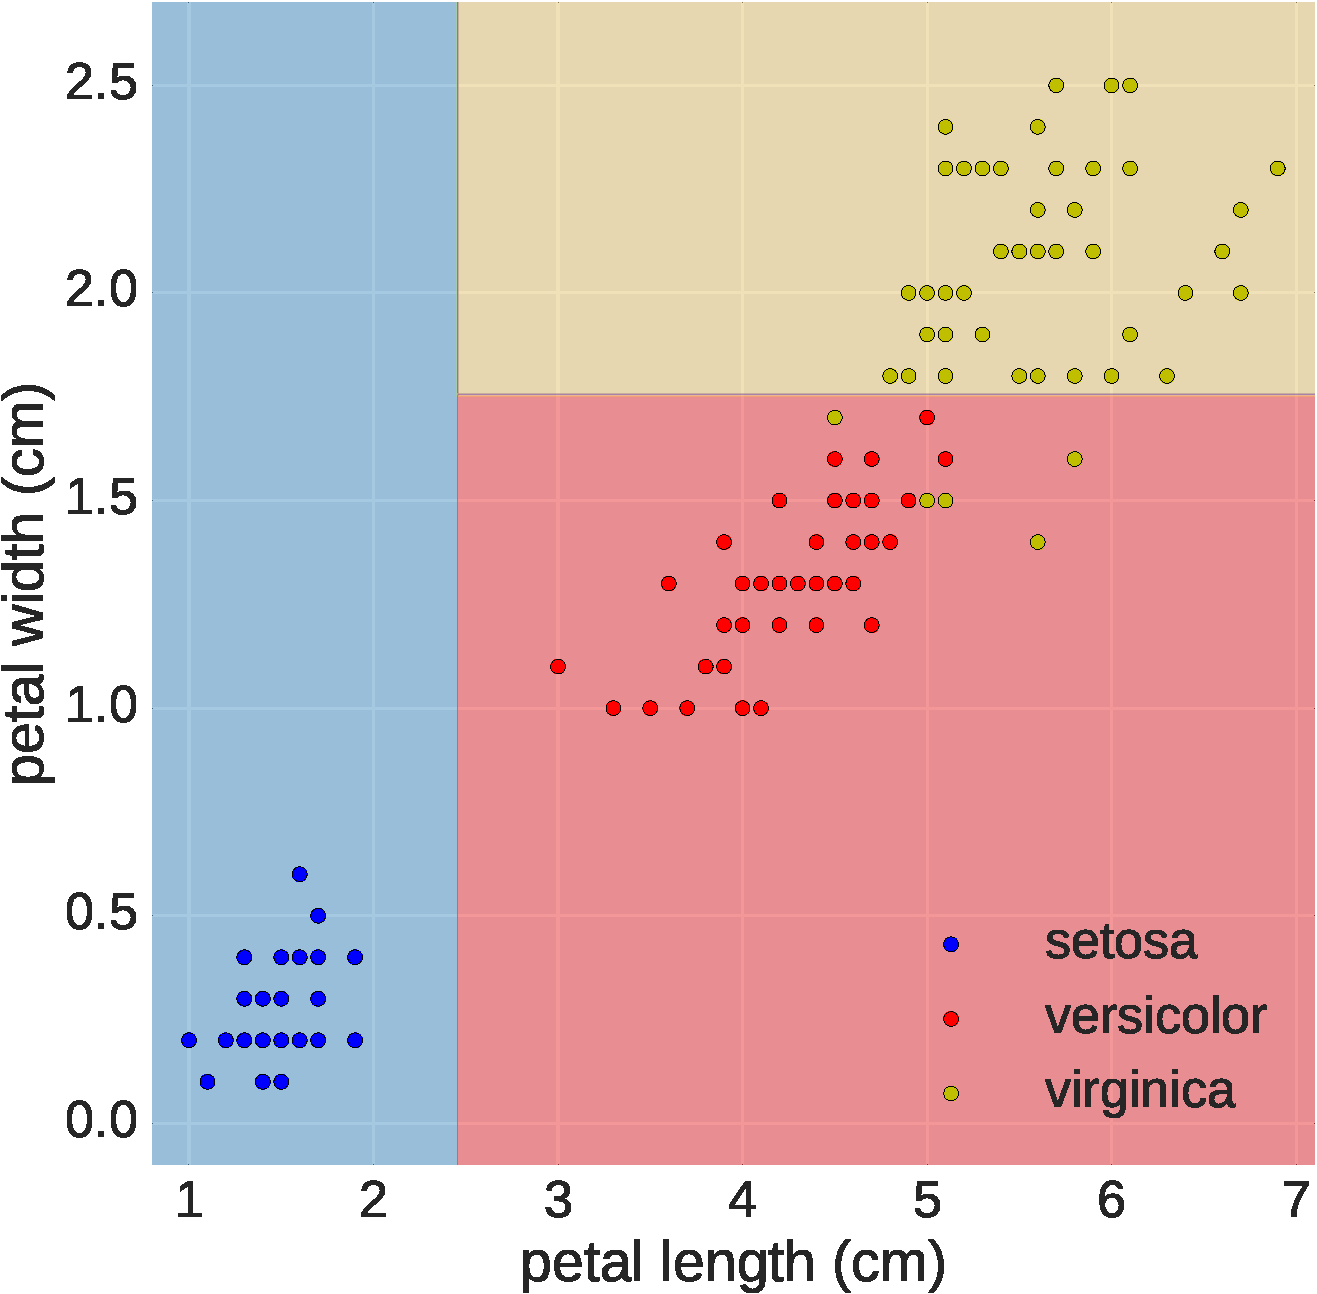
\includegraphics[width=\textwidth]{../fig/iris_ds-crop.pdf}
\column{0.5\textwidth}
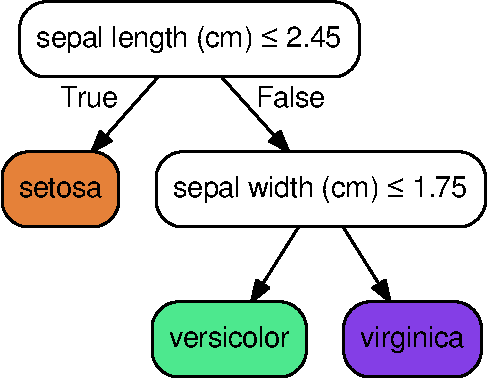
\includegraphics[width=\textwidth]{../fig/iris_dt-crop.pdf}
\end{columns}
\end{frame}
\end{document}